\documentclass[border=10px]{standalone}
\usepackage{tikz}
\usepackage[european]{circuitikz}


\begin{document}
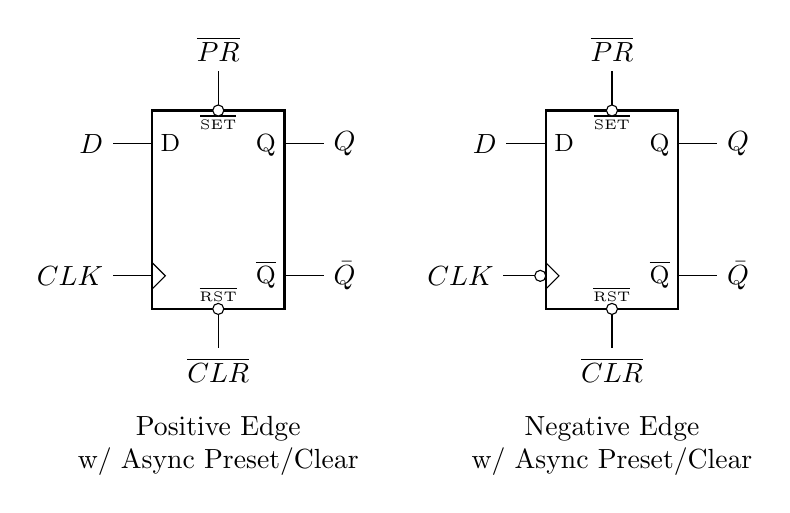
\begin{tikzpicture}
    % Positive Edge D-FF with Async Reset/Preset
    \node [flipflop D, add async SR, external pins width=0] (FF1) at (0,0) {};
    \draw (FF1.pin 1) -- ++(-0.5,0) node[left] {$D$};
    \draw (FF1.pin 3) -- ++(-0.5,0) node[left] {$CLK$};
    \draw (FF1.pin 6) -- ++(0.5,0) node[right] {$Q$};
    \draw (FF1.pin 4) -- ++(0.5,0) node[right] {$\bar{Q}$};
    % Async pins are typically active low bubbles in recent circuitikz if styled, 
    % but 'add async SR' just adds the pins. We can match standard symbol by adding bubbles or text overbars.
    % Let's assume standard behavior. Bubbles are often manual or dependent on style.
    % Adding manual bubbles if needed, or just text.
    \draw (FF1.up) -- ++(0,0.5) node[above] {$\overline{PR}$};
    \draw (FF1.down) -- ++(0,-0.5) node[below] {$\overline{CLR}$};
    
    \node [below=2.5cm, align=center] at (FF1) {Positive Edge \\ w/ Async Preset/Clear};

    % Negative Edge D-FF
    \node [flipflop D, add async SR, external pins width=0] (FF2) at (5,0) {};
    \draw (FF2.pin 1) -- ++(-0.5,0) node[left] {$D$};
    % Manual bubble for negative edge clock
    \draw [fill=white] (FF2.pin 3) ++(-2pt,0) circle(2pt);
    \draw (FF2.pin 3) ++(-4pt,0) -- ++(-0.4,0) node[left] {$CLK$};
    
    \draw (FF2.pin 6) -- ++(0.5,0) node[right] {$Q$};
    \draw (FF2.pin 4) -- ++(0.5,0) node[right] {$\bar{Q}$};
    \draw (FF2.up) -- ++(0,0.5) node[above] {$\overline{PR}$};
    \draw (FF2.down) -- ++(0,-0.5) node[below] {$\overline{CLR}$};

    \node [below=2.5cm, align=center] at (FF2) {Negative Edge \\ w/ Async Preset/Clear};

    % Manually adding bubbles for PR/CLR if circuitikz didn't (it might not by default on the stick)
    % A small circle at the connection point
    \draw [fill=white] (FF1.up) circle(2pt);
    \draw [fill=white] (FF1.down) circle(2pt);
    \draw [fill=white] (FF2.up) circle(2pt);
    \draw [fill=white] (FF2.down) circle(2pt);

\end{tikzpicture}
\end{document}
